\section{Framework}
\label{sec:framework}

Our framework has four main components: Path generation, Path searching, Schedule and Transport as depicted in Figure \ref{fig:framework}. 
\begin{figure}[!htb]
\vspace{-0.15in}
\centering
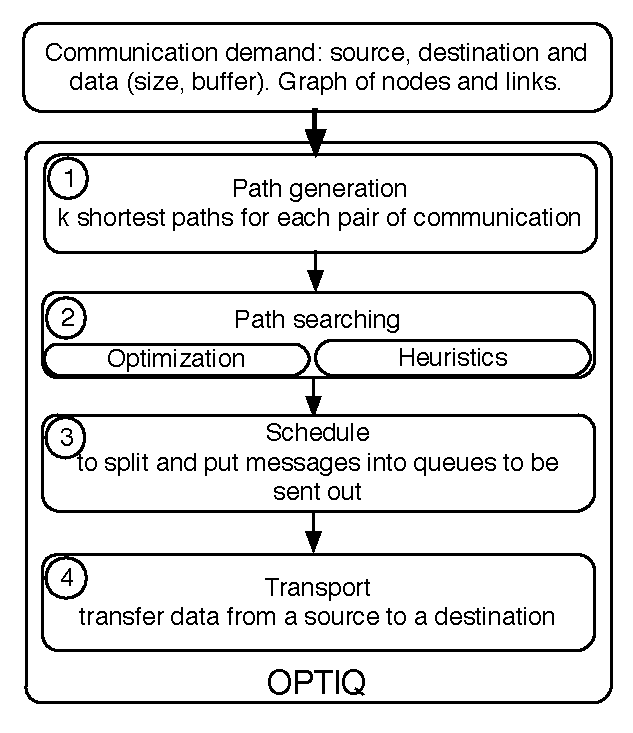
\includegraphics[scale=0.5]{figures/framework.pdf}
\vspace{-0.15in}
\caption{\small Four components of OPTIQ framework}
\vspace{-0.15in}
\label{fig:framework}
\end{figure}
The functionality of each component is as follows:
\begin{itemize}
\item Path generation: generate k shortest paths that can be used as candidates for data transfer. We need to generate paths to reduce the search space.
\item Path searching: search for paths to transfer data from a set of sources to a set of destinations. Multiple paths or a single path can be found using a set of approaches. User can use one of the approaches provided by the framework or can add their own approaches.
\item Schedule: Split data buffer that needs to be transferred into smaller messages and put those messages into a queue of the Transport layer to be transferred. It also handles the order of sending and forwarding messages.
\item Transport: actually transfer data from one node to another in the system. As data moves along a path, we need to copy data at each intermediate node on the path and inject the data to the network to be transferred to the next destination on the path.
\end{itemize}
The framework has various options to allow users to tune the framework for optimal performance, such as order of sending or forwarding messages, choosing path searching algorithms, setting chunk size to transfer messages. 

Applications use the framework via a simple application programming interface (API). The framework handle data movement for the applications. The framework takes inputs from applications such as data sizes, data buffers, communication patterns. It also read system's information such as topology, compute nodes' coordinates as input for paths computation. The framework searches for paths either online or offline. After paths is found, data is split among all paths and is transferred along paths from sources to destinations. The data is transferred from sources to intermediate nodes on the paths to destinations. Extra time for data copy and injection incurs at intermediate nodes. We use pipeline to reduce this time. The framework splits messages at the source nodes and assembles messages at the destinations node based on their source nodes and offsets.
